\section{Exploratory probes in full}
\label{app:probes}

We ran three single-seed follow-up runs, each aimed at another possible cause of the main result:
an objective that rewards constant behavior, too little data, and a model without spatial grounding.
Section~\ref{sec:probes} summarizes them, and this appendix gives the protocol and the confounds.
These probes are exploratory. They were planned after the main results, each has one seed,
and all three share the loader confound described under Probe~1. Each was verified by independent
reconstruction from raw per-decision or per-episode artifacts, and every number below is generated
from those artifacts.

\paragraph{Probe 1: supervise four-action chunks.}
Under single-action supervision, always predicting \textsc{move\_forward} matches
\PrConstSingle\% of released training decisions. Re-rendering supervision as four-action chunks
cuts the best constant strategy to \PrConstChunk\% of exact chunks. The loss, however, is a mean
over chunk positions, and a constant \textsc{move\_forward} still matches $68.0\%$ of the positions
this probe trained on. The backbone, adapter configuration, optimizer settings, observation cache,
partitions and seed match the main study, but the budget is larger. This probe ran
\PrPilotUpdates{} updates, about \PrPilotEpochs{} epochs against the main study's single epoch. The
rolled-out checkpoint is update \PrPilotCkptU, selected on the same frozen selection set. Because the
long run kept only its final state, that checkpoint comes from a re-run stopped at \PrPilotCkptU{}
updates (selection CE $0.6793$). The probe also supervises four token positions per decision where the
original supervised one. Because a chunk needs four future actions, the loader drops every cached
decision in a trajectory's last three steps, including every decision whose target is
\textsc{stop}. \textsc{stop} is therefore supervised only as a chunk's fourth action, and the
selection set keeps $240$ of its $256$ decisions. Across the chunk runs, \textsc{stop} is
$0.47$--$0.57\%$ of supervised positions, against $2.31\%$ of the main-study training decisions, and
$4$ of the $960$ positions on the selection set. No chunk run is trained to emit \textsc{stop} as its
next action, so this pipeline largely produces policies that never stop. In the simulator, the
policy uses all three movement actions, and constant-action episodes fall from $61/61$ to
\PrPilotClConst$/61$. It emits \PrPilotClStopActs{} \textsc{stop} actions in \PrPilotClActs{}
executed actions. The probe changes the objective, the supervision density and the budget together,
so it does not isolate any one of them.

\paragraph{Probe 2: scale the data 44$\times$.}
We expanded the frozen 3{,}072-decision training set to \PrFortyN{} and then \PrBigN{} decisions.
The sets are \emph{nested}: each contains the frozen list as a verified position-for-position
prefix, drawn from the same 2{,}451 trajectories under the same eligibility rules and seed, so the
contrast isolates the number of unique decisions. The update budget is held at 3{,}000, so the
number of epochs falls. After the chunk filter, the two runs train on $37{,}627$ and $127{,}661$
samples, and each run's $48{,}000$ sample draws come to $1.28$ and $0.38$ epochs. The best selection
cross-entropy is \PrPilotMinCE{} for the chunk run, \PrFortyMinCE{} at \PrFortyN{} decisions and
\PrBigMinCE{} at \PrBigN{}. The chunk run's value comes from the longer schedule above and is not
budget-matched to the two scaled runs, and each value is one seed, so we do not rank the three.
Held-out accuracy reaches \PrBigAccHi{} against an always-forward reference of \PrAfAcc{} on the
same set. Across all \PrFortyPts{} and \PrBigPts{} calibration points (checkpoints scored on the
selection set during training) of the two scaled runs, \textsc{stop} was predicted
\PrFortyStopTot{} and \PrBigStopTot{} times. The chunk run's \PrPilotStopTot{} scattered \textsc{stop}
predictions, three of them correct, occur only after two epochs, in an overfitting regime that the
scaled runs never enter, so we make no causal claim about scale removing them. In the simulator, the
largest run's checkpoint enters the goal radius on \PrBigClOracle$/61$ episodes
(Figure~\ref{fig:probe_trajectories}) and emits \PrBigClStopActs{} \textsc{stop} actions in
\PrBigClActs{} actions.

\begin{figure}[t]
  \centering
  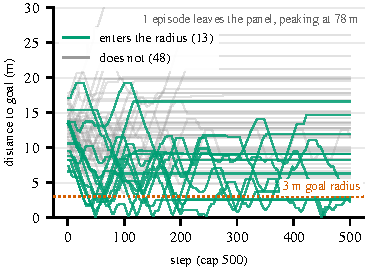
\includegraphics[width=0.5\linewidth]{figures/p1_trajectories.pdf}
  \caption{\textbf{The largest probe run in closed loop.} Distance to goal over the $500$-step cap
  for the $61$ episodes of the exploratory $134{,}754$-decision run of Probe~2, whose chunk loader
  (Probe~1) dropped every decision whose target was \textsc{stop}. Green enters the $3$\,m radius, grey does not.
  Thirteen of the $61$ enter it, against the $1/61$ Oracle Success every main-study checkpoint
  records in Table~\ref{tab:closed-loop-behavior}. No episode ends with \textsc{stop}.}
  \label{fig:probe_trajectories}
\end{figure}

\paragraph{Probe 3: inject explicit metric geometry.}
We attached a geometry branch to the frozen backbone at the largest budget. The simulator's
ground-truth metric depth for each frame is backprojected through the camera model and aggregated
to 64 patch points per frame, with invalid pixels masked. An equivariant geometric-algebra
transformer processes these points through a readout that preserves metric scale and egocentric
direction, and its output enters the model as 256 additional tokens whose attention phases carry a
multi-scale 3D positional code (wavelengths 0.60--12\,m). Replacing real depth with a flat wall
shifts the branch's output by \PrGeoWall{} of its own standard deviation at the selected checkpoint,
so the branch carries information about the scene. The
model also uses it: masking the tokens at fixed weights moves selection cross-entropy from
\PrGeoMinCE{} to \PrGeoMasked. Trained on the same data, adapter, seed, budget and selection set as
the geometry-free run, plus the branch's own $17.6$M parameters at learning rate $10^{-4}$, the
geometry arm reached \PrGeoMinCE{} against the geometry-free baseline's \PrBigMinCE{} at the same
budget. Both values are single-seed and fall on the last scored checkpoint, and seed variation alone
can separate learning curves that share a configuration \citep{henderson2018matters}. The geometry
arm predicted \textsc{stop} \PrGeoStopTot{} times across \PrGeoPts{} calibration points, and in the
simulator it entered the goal radius on \PrGeoClOracle$/\PrGeoClEps$ episodes while emitting
\PrGeoClStopActs{} \textsc{stop} actions in \PrGeoClActs{} actions. Published results on depth or 3D
input to VLM navigation policies point in both directions. Adding simulator depth to a fine-tuned
VLM lowered R2R-CE \texttt{val\_unseen} success from $27.1$ to $23.1$, which the authors attribute to
the model's limited ability to process depth \citep{zhang2025mapnav}. Entity-level 3D soft tokens
injected into a frozen VLM improved object-goal navigation \citep{softnav2026}. We know of no
measurement of the configuration used here, per-patch metric-depth geometry tokens with a
multi-scale 3D positional code on an instruction-following R2R-CE policy. This single-seed result
adds one data point to a mixed record.

\paragraph{Summary and limits.}
Each probe changed one mechanism that could explain the constant-action behavior (the objective's
payoff, the amount of data, the lack of spatial structure), and behavior changed. Constant-action
episodes fell, the largest run entered the goal radius far more often, and the model used the
geometry tokens. These results do not bear on stopping. Summed over every calibration point of the
scaled and geometry runs, \textsc{stop} was predicted \PrFortyStopTot{} times at 13$\times$ data,
\PrBigStopTot{} at 44$\times$, and \PrGeoStopTot{} with geometry, but the loader described under
Probe~1 removed every \textsc{stop}-target decision from training and selection. These zeros, like
the absence of \textsc{stop} in the simulator, are therefore largely a product of the pipeline, and
the probes cannot show that the selection loss's blindness to \textsc{stop} persists under these
changes. Each probe is one seed at one configuration and was planned after the main results. The
134k and geometry runs reach their lowest selection cross-entropy at their final calibration point
(the 40k run's minimum is interior, at update \PrFortyMinU{} of 3{,}000), so no convergence claim is
available for the two largest runs. The geometry probe adapts the frozen backbone only through a
rank-32 attention-only adapter, a configuration no VLN-CE system we know of reports using, and it
reads the simulator's ground-truth depth, so it bounds only this configuration.
